\documentclass[11pt]{article} % Increase font size slightly
\usepackage{graphicx}
\usepackage{hyperref}
\usepackage{geometry}
\usepackage{amsmath} % For math environments if needed later
\usepackage{enumitem} % For better list control
\geometry{a4paper, margin=1in}

% Set up the images directory path
\graphicspath{{images/}}

% Create a custom command for the logo
\newcommand{\plansynclogo}[1][\textwidth]{%
    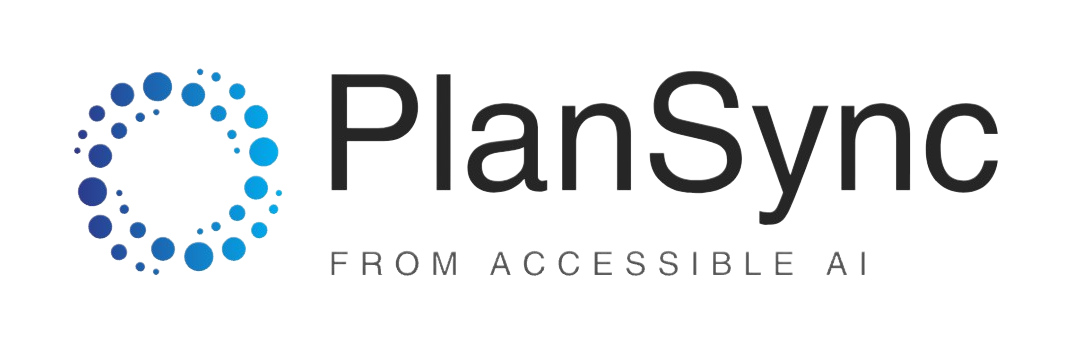
\includegraphics[width=#1]{logo.png}
}

\title{
    \plansynclogo[0.4\textwidth]
    \vspace{1cm}
    
    PlanSync AI: Revolutionizing 401(k) Plan Management \\ 
    \large An In-depth Analysis for Financial Advisors
}
\author{PlanSync AI Team}
\date{\today}

\begin{document}

\maketitle

\begin{abstract}
\noindent The management of 401(k) retirement plans presents escalating complexities for financial advisors, driven by stringent regulatory requirements, vast data volumes, and increasing client expectations. Effective management, robust compliance, and insightful reporting are not merely administrative functions but core fiduciary responsibilities. Manual processes are often inefficient, error-prone, and costly, hindering advisors\' ability to provide strategic value and increasing operational and legal risks. PlanSync AI offers a specialized Customer Relationship Management (CRM) platform enhanced with Artificial Intelligence (AI) to specifically address these critical challenges. This white paper details the mission-critical nature of compliance, data integrity, and reporting for 401(k) advisors, outlines the architecture and features of PlanSync AI designed to bolster these functions, demonstrates its benefits through practical use cases, addresses crucial data security considerations, and concludes on its transformative potential for the advisory practice. By automating compliance tasks, centralizing data intelligence, and streamlining reporting, PlanSync AI empowers advisors to enhance efficiency, demonstrably mitigate risk, and focus on high-value client engagement.
\end{abstract}

\section{Introduction}
The landscape of employer-sponsored retirement plans, particularly 401(k)s, is characterized by increasing complexity and demanding regulatory oversight. Financial advisors serving this market are pivotal in guiding plan sponsors and participants, fulfilling crucial fiduciary duties that hinge upon meticulous data management, unwavering compliance, and transparent reporting. These are not optional activities; they form the bedrock of trust and legal soundness in the advisor-client relationship. The sheer volume of data associated with multiple plans, coupled with the constant evolution of regulations from bodies like the Department of Labor (DOL) and the Internal Revenue Service (IRS), creates an environment where lapses can have severe consequences. Traditional CRM systems and manual processes often fall short, lacking the specialized functionality needed for efficient and, more importantly, *defensible* 401(k) plan management. PlanSync AI emerges as a purpose-built solution, leveraging Artificial Intelligence to automate, streamline, and enhance the capabilities of 401(k) advisors, transforming their operational challenges into strategic advantages built on a foundation of rigorous compliance and data integrity.

\section{The Challenge: Navigating Complexity and Risk in 401(k) Plan Management}
Advisors specializing in 401(k) plans face a unique confluence of challenges where operational efficiency directly intersects with fundamental fiduciary responsibility and risk management:
\begin{itemize}[leftmargin=*]
    \item \textbf{Intensive Data Management Demands Absolute Accuracy:} Advisors must track a multitude of data points across diverse plans and participant demographics. This includes contribution rates, investment allocations, loan details, distributions, eligibility tracking, and beneficiary information. Errors or inconsistencies in this data are not just inconvenient; they can lead to incorrect reporting, failed compliance tests, and potential fiduciary breaches. Managing this data fragmented across spreadsheets, legacy systems, or generic CRMs is not only inefficient but dangerously increases the risk of data silos, inconsistencies, and ultimately, costly mistakes.
    \item \textbf{Crushing Regulatory Burden with Zero Tolerance for Error:} Compliance is non-negotiable and requires constant vigilance. Key regulations like the Employee Retirement Income Security Act (ERISA) impose strict fiduciary duties, holding advisors personally liable for acting in the best interests of plan participants. Advisors must navigate complex requirements related to non-discrimination testing (ADP/ACP), fee disclosures (408(b)(2)), participant notices, timely Form 5500 filings, and meticulous adherence to plan documents. Staying updated and ensuring consistent, documented application across all client plans is paramount. Failure to comply is not an option and can result in substantial penalties from the DOL/IRS, participant lawsuits, disqualification of the plan, and irreparable reputational damage.
    \item \textbf{Reporting Inefficiencies Undermine Value and Increase Risk:} Generating routine and ad-hoc reports for compliance documentation, plan reviews, and client meetings is a critical function, not just an administrative task. These reports are evidence of due diligence and proper plan stewardship. Manual compilation is not only laborious and susceptible to human error but also fails to provide timely insights. This detracts from client-facing activities and increases the risk that potential issues are not identified and addressed promptly. The time spent on these essential administrative tasks directly impacts profitability and the advisor\'s capacity for growth.
    \item \textbf{Need for Proactive Insights to Fulfill Fiduciary Duty:} Beyond basic administration, fulfilling a fiduciary role requires advisors to provide strategic guidance based on accurate data. Identifying plans at risk of compliance failures *before* they occur, spotting opportunities for plan design improvements to benefit participants, or analyzing participant behavior trends to enhance outcomes are essential aspects of modern advisory. These require analytical capabilities often lacking in traditional workflows, hindering the advisor's ability to proactively serve their clients' best interests.
\end{itemize}

\section{The Solution: PlanSync AI - An Intelligent CRM}
PlanSync AI is engineered from the ground up as an intelligent CRM specifically for the 401(k) advisory market. It moves beyond simple data storage to provide a dynamic platform for efficient management, compliance assurance, and data-driven insights.

\begin{figure}[htbp]
    \centering
    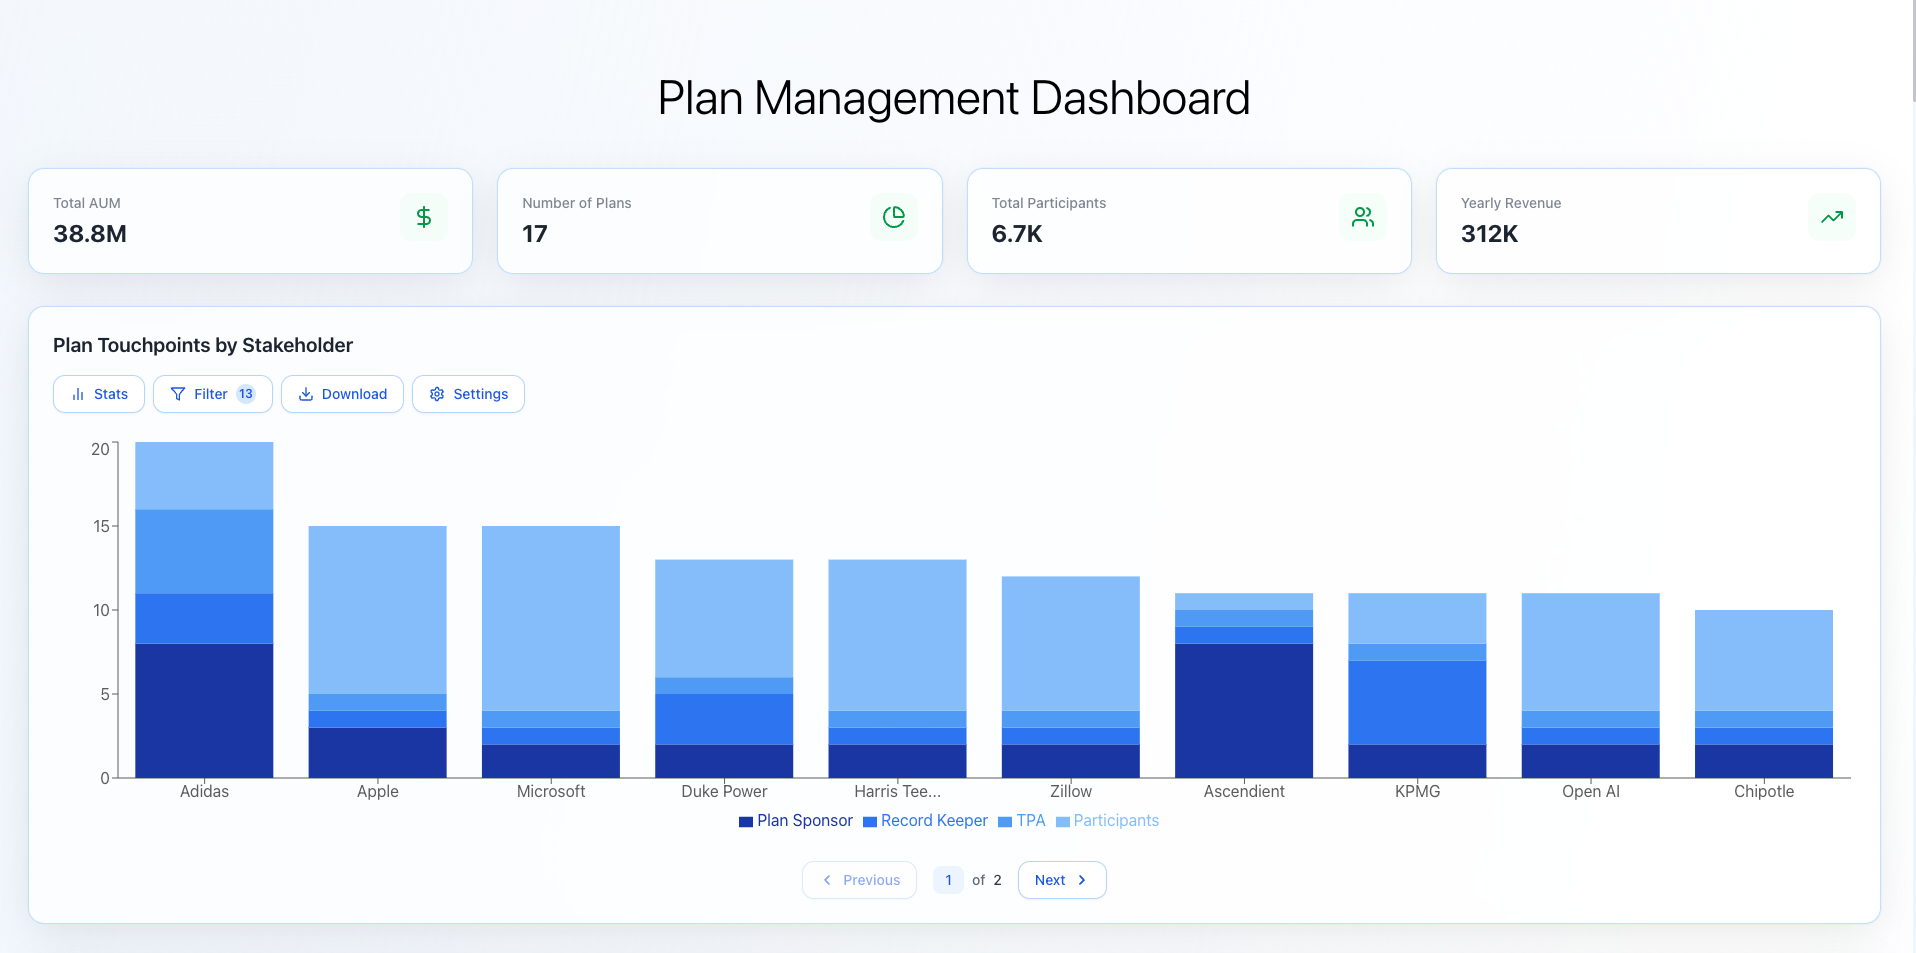
\includegraphics[width=0.9\textwidth]{dashboard.png}
    \caption{PlanSync AI's intuitive dashboard provides a comprehensive overview of plan health, compliance status, and key metrics.}
    \label{fig:dashboard}
\end{figure}

By integrating advanced AI algorithms, PlanSync AI automates routine tasks, proactively identifies potential issues, and centralizes all plan-related information and workflows.

\subsection{Core Architecture Principles}
While the specific AI models are proprietary, the platform operates on principles including:
\begin{itemize}[leftmargin=*]
    \item \textit{Centralized Data Hub:} Aggregating data from various sources (recordkeepers, payroll providers, plan documents) into a unified, structured database.
    \item \textit{Rule-Based Engines:} Encoding regulatory requirements and best practices to automate compliance checks and alerts.
    \item \textit{Machine Learning Capabilities:} Analyzing historical and current data to identify patterns, predict potential compliance issues (e.g., testing failures), and surface actionable insights for advisors.
    \item \textit{Natural Language Processing (NLP):} Potentially used for analyzing plan documents or summarizing regulatory updates (future capability).
\end{itemize}

\section{Key Features In-Depth}
PlanSync AI provides a robust feature set designed to directly address advisor pain points:

\begin{figure}[htbp]
    \centering
    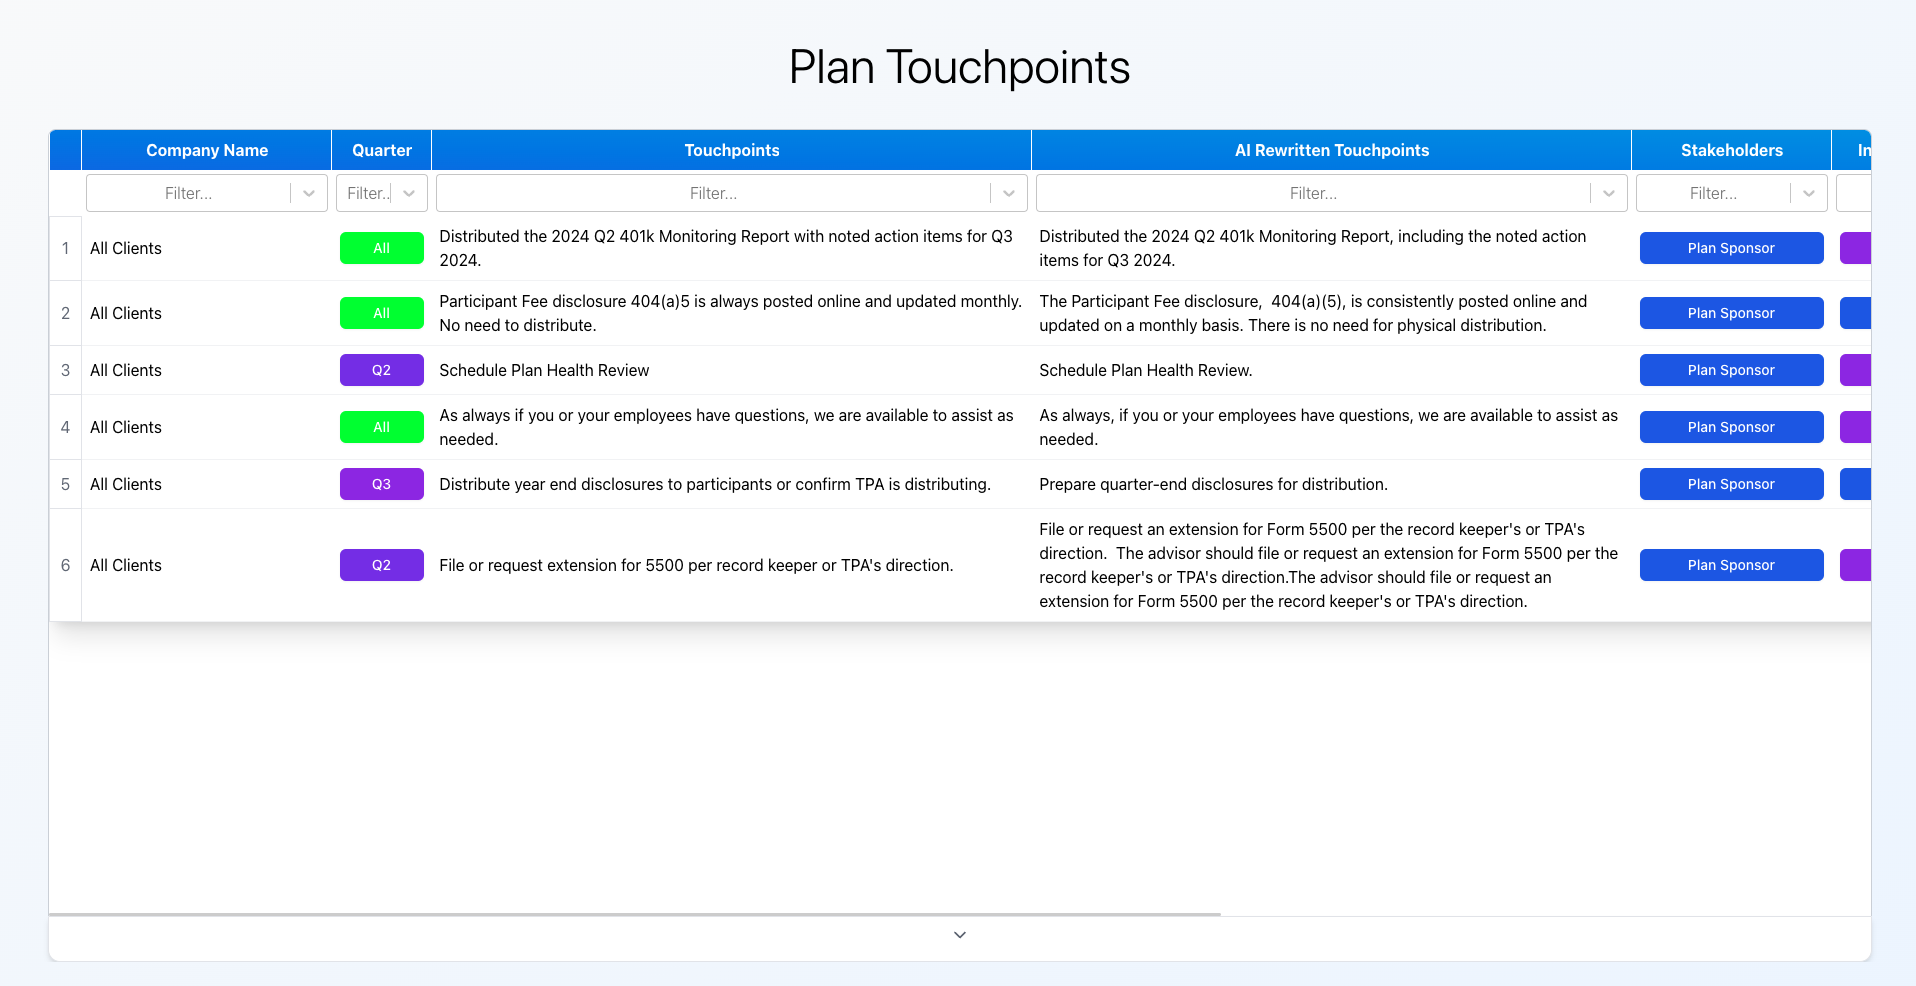
\includegraphics[width=0.85\textwidth]{features.png}
    \caption{The PlanSync AI Master Spreadsheet centralizes critical plan data for efficient management and analysis.}
    \label{fig:features}
\end{figure}

\begin{itemize}[leftmargin=*]
    \item \textbf{Intelligent Data Management & Analytics:} 
        \begin{itemize}[label=\textbullet, leftmargin=*]
            \item Unified dashboard providing a holistic view of all managed plans.
            \item Centralized repository for plan documents, census data, investment information, and communication logs.
            \item AI-powered analytics to track key plan health indicators, participation rates, contribution trends, and potential compliance red flags.
            \item Automated data validation and anomaly detection to ensure data integrity.
        \end{itemize}
    \item \textbf{Automated Compliance Workflows:} 
        \begin{itemize}[label=\textbullet, leftmargin=*]
            \item Proactive alerts for critical compliance deadlines (e.g., Form 5500, required notices).
            \item Automated checks against common compliance pitfalls based on integrated regulatory rules.
            \item Streamlined data gathering and preparation assistance for non-discrimination testing (NDT) and Form 5500 filings.
            \item Centralized tracking of fee disclosures and service agreements.
        \end{itemize}
    \item \textbf{Instant Compliance Report Generation:} 
        \begin{itemize}[label=\textbullet, leftmargin=*]
            \item On-demand generation of standardized and customizable reports (e.g., Annual Plan Review summaries, Compliance Checklists, Fee Benchmarking data prep).
            \item Ability to generate reports across multiple plans simultaneously.
            \item Reduces report preparation time from hours or days to minutes, ensuring accuracy and consistency.
        \end{itemize}
\end{itemize}

\section{Use Cases: PlanSync AI in Action}
To illustrate the practical impact, consider these scenarios:
\begin{itemize}[leftmargin=*]
    \item \textbf{Scenario 1: Proactive Compliance Management:} Advisor Sarah manages 70 plans. PlanSync AI automatically flags five plans potentially at risk of failing ADP/ACP testing based on mid-year census data analysis. Sarah receives an alert, reviews the detailed projections within the platform, and proactively contacts the sponsors to discuss corrective strategies well before year-end, preventing costly corrective distributions.
    \item \textbf{Scenario 2: Efficient Annual Reviews:} Advisor John needs to prepare for 15 annual plan review meetings in the next month. Using PlanSync AI, he instantly generates comprehensive review packages for each client, including compliance summaries, plan health metrics, participation statistics, and fee benchmark comparisons. This saves him days of manual data aggregation and allows him to focus on strategic discussions during the meetings.
    \item \textbf{Scenario 3: Streamlining Form 5500 Preparation:} Advisor Emily's team typically spends weeks coordinating data gathering for Form 5500 filings. PlanSync AI centralizes much of the required data and provides checklists and workflow tools, significantly reducing the administrative burden and minimizing the risk of late filing penalties.
\end{itemize}

\section{Data Security and Privacy}
PlanSync AI recognizes the critical importance of protecting sensitive plan and participant data. Our platform is built with robust security measures:

\begin{figure}[htbp]
    \centering
    
\includegraphics[width=0.5\textwidth]{security.png}
    \caption{PlanSync AI implements enterprise-grade security protocols to protect sensitive plan and participant data.}
    \label{fig:security}
\end{figure}

\begin{itemize}[leftmargin=*]
    \item \textbf{Encryption:} Data is encrypted both in transit (using TLS/SSL) and at rest (using industry-standard algorithms like AES-256).
    \item \textbf{Access Controls:} Role-based access controls ensure that users only have access to the information necessary for their roles. Multi-factor authentication (MFA) is enforced.
    \item \textbf{Infrastructure Security:} Hosted on secure cloud infrastructure (e.g., AWS, Azure, GCP) adhering to rigorous security standards (SOC 2, ISO 27001).
    \item \textbf{Regular Audits:} Periodic security audits and penetration testing are conducted by third-party experts.
    \item \textbf{Compliance with Privacy Regulations:} Designed to help advisors comply with relevant data privacy laws (e.g., GDPR, CCPA where applicable).
\end{itemize}

\section{Benefits for Advisors Revisited: Enhancing Value Through Diligence}
The adoption of PlanSync AI translates into significant advantages that reinforce the core tenets of responsible advisement:
\begin{itemize}[leftmargin=*]
    \item \textbf{Drastic Efficiency Gains to Reinvest in Client Value:} Automating data management, compliance checks, and reporting frees up significant advisor and staff time. This isn't just about cost savings; it's about redirecting resources towards strategic plan consulting, participant education, and relationship building – activities that directly demonstrate advisor value.
    \item \textbf{Demonstrably Mitigated Compliance Risk:} Proactive alerts and automated checks provide a systematic approach to compliance, substantially reducing the likelihood of costly errors, fines, and fiduciary breaches. This documented diligence is crucial in the event of an audit or dispute.
    \item \textbf{Enhanced Data Accuracy and Integrity as a Foundation:} Centralization and automated validation minimize errors associated with manual data entry and disparate systems, ensuring that advice and reporting are based on reliable information – a cornerstone of fiduciary responsibility.
    \item \textbf{Improved Client Service, Trust, and Retention:} Faster response times, proactive identification of issues, documented compliance procedures, and more strategic review meetings build and solidify client trust and strengthen relationships.
    \item \textbf{Scalability and Growth on a Secure Foundation:} Reduced administrative burden and enhanced risk management allow advisors to confidently scale their practice, knowing their core compliance and data responsibilities are systematically managed.
\end{itemize}

\section{Conclusion}
PlanSync AI is more than just a CRM; it is an intelligent ecosystem designed to support the critical responsibilities inherent in the 401(k) advisory market. By tackling the core challenges of data management, regulatory compliance, and reporting inefficiency through AI-driven automation and insights, it fundamentally strengthens an advisor's ability to meet their fiduciary obligations. PlanSync AI empowers advisors to move beyond reactive administration towards proactive, documented, and strategic guidance, ultimately enhancing their value proposition, demonstrably reducing operational and legal risk, and paving the way for sustainable practice growth built upon a foundation of trust and diligence in an increasingly complex retirement landscape.

\end{document} 